\chapter{Introduction}
\gls{rails} is a software model and implementation of an automated system to assist the model railroader achieve realism in the operation of a model railroad. The model then drives the development of hardware and or software.
\section{Microservices Design Components}
Figure \ref{fig:microarchitecture} shows the microservices components that make up the design of \gls{rails}.

\begin{figure}[H]
	\centering
		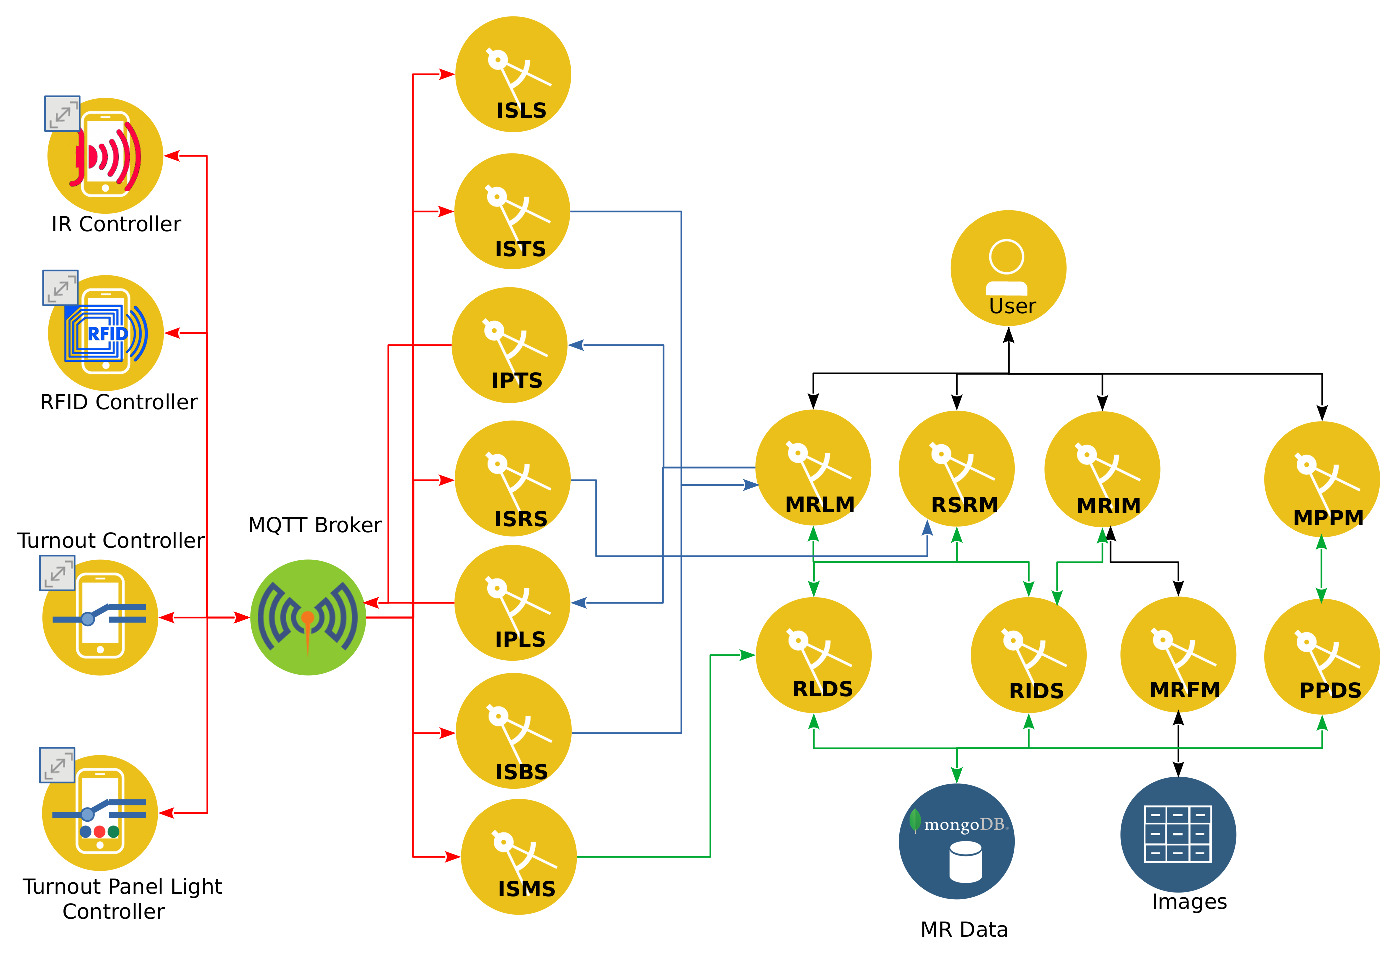
\includegraphics[scale=0.7]{../System/design.eps}
	\caption{Microservices Component Architecture}
	\label{fig:microarchitecture}
\end{figure}

The microservices design components are divided into three sets:
\begin{itemize}
  \item \gls{iot} components, which are highlighted with the light green colored background in Figure \ref{fig:microarchitecture}.
  \item \gls{ds} components, which are highlighted with the light blue colored background in Figure \ref{fig:microarchitecture}.
  \item \gls{spa} components, which are highlighted with the buff colored background in Figure \ref{fig:microarchitecture}.
\end{itemize}

\subsection{IoT Components}
The components of the \gls{iot} set of design components are subdivided into:
\begin{itemize}
  \item Micro Controllers using the \gls{mqtt} protocol:
\begin{itemize}
  \item \gls{rfid} Controller processes \gls{rfid} tags obtained from a \gls{rfid} reader and then publishes the value
  \item Turnout Controller subscribes to turnout commands then to act on the command to cause the turnout to move. It then publishes the state of the turnout
  \item \gls{ir} Controller (in planning) processes \gls{ir} sensors and publishes their values
\end{itemize}
  \item \gls{mqtt} Broker is the heart of any publish/subscribe protocol, is responsible for receiving messages, posting to designated topics and sending messages to clients subscribing to topics.
  \item The subscribers and publishers bridge the \gls{mqtt} elements with the \gls{gui} applications:
\begin{itemize}
  \item \gls{ipls} publishes turnout panel light commands a Turnout Panel Controller
  \item \gls{ipts} publishes turnout commands to a Turnout Controller
  \item \gls{isbs}  subscribes to push button events and pushes them via a web-socket to the MRLM component
  \item \gls{isls} (in planning) \gls{iot} subscribes to topics that provide location information i.e., \gls{ir} Sensors and \gls{rfid} sensors
  \item \gls{isms} subscribes to micros and adds or updates micros collection in \gls{rails}. It also subscribes to micro heartbeats.
  \item \gls{isrs} subscribes to \gls{rfid} tags and pushes them via a web-socket to the \gls{rsrm} component
  \item \gls{ists} subscribes to turnout switch closures and pushes them via a web-socket to the \gls{mrlm} component
\end{itemize}
\end{itemize}
\subsection{DS Components}
\gls{ds} consist of all the components that handle and or store the model railroad data:
\begin{itemize}
  \item MR Data – the document repository, MongoDB, to store complete collections of items such as rolling stock, industries (producers and consumers), track elements, turnouts, projects, purchases, etc.
  \item \gls{rids} provides \gls{rest} access to railroad inventory documents
  \item \gls{ppds} provides \gls{rest} access to model railroad projects and purchases documents
  \item \gls{rlds} provides \gls{rest} access to model railroad layout documents
  \item \gls{mrfm} provides the user the ability to upload image files for the use by the \gls{mrim} component
  \item Images is the file store for the images uploaded by \gls{mrfm} component and used by the \gls{mrim} component
\end{itemize}
\subsection{SPA Components}
\gls{gui} applications that provide user access to \gls{rails}:
\begin{itemize}
  \item \gls{rsrm}, this \gls{spa} allows a user to match a \gls{rfid} value to a rolling stock road name and number
  \item \gls{mrim}, this \gls{spa} allows a user to create, update and delete model railroad assets, such as rolling stock
  \item \gls{mppm}, this \gls{spa} allows a user to enter information about their projects and purchases
  \item \gls{mrlm}, this \gls{spa} allows a user to enter information about their layout and control elements of it
\end{itemize}
\section{Docker}
In the context of microservices, containers are used to package the code, libraries, and configuration files needed for a microservice to run as a single, executable unit. This makes it easy to deploy and run microservices in different environments, such as on-premises servers or in the cloud. By packaging all the dependencies for a microservice in a container, it can be guaranteed to run the same way regardless of the environment it's deployed in. This helps to reduce issues caused by differences between development, testing, and production environments. Containers also make it easy to scale up or down the number of instances of a microservice running, and to update or rollback a microservice without affecting other services.\vspace{5mm} \\
Docker is a platform that makes it easy to create, deploy, and run applications in containers. It provides a \gls{cli} and a set of \glspl{api} that make it simple to work with containers. Docker in conjunction with microservices is used to package and deploy each service in its own container. This allows each service to be managed, deployed, and scaled independently of other services. The Docker platform provides a number of tools to help manage and orchestrate the containers that make up a microservice-based application, such as Docker Compose and Docker Swarm.\vspace{5mm} \\
Docker is an open-source platform that enables developers to automate the deployment, scaling, and management of applications using containerization. Containers are lightweight, isolated environments that encapsulate an application and all its dependencies, including libraries, frameworks, and other runtime components. Docker allows the user to package an application into a container image, which can then be run consistently across different environments, such as development, testing, and production.\vspace{5mm} \\
Docker provides the following features:
\begin{itemize}
  \item Docker containers are portable and can run on any system that supports Docker, regardless of the underlying operating system or infrastructure. This eliminates the "works on my machine" problem and ensures consistent behavior across different environments.
  \item Containers provide a high level of isolation, ensuring that applications and their dependencies are encapsulated and do not interfere with each other. This isolation improves security, as well as prevents conflicts between different software components.
  \item Docker containers are lightweight and share the host system's operating system kernel. This means they require fewer resources compared to traditional \glspl{vm}. Multiple containers can run on the same host without significant performance overhead.
  \item Docker makes it easy to scale applications horizontally by running multiple instances of containers across different hosts or a cluster of machines. This enables efficient utilization of resources and helps handle increased workload demands.
  \item Docker allows versioning of container images, making it easier to track changes and roll back to a previous version if needed. This simplifies the deployment and update process, reducing the risk of application downtime.
  \item Docker has a large and active community, resulting in a vast ecosystem of pre-built container images available from Docker Hub and other registries. These images can be easily pulled and used as a base for building and deploying applications, saving development time.
\end{itemize}
The key aspects of Docker are:
\begin{itemize}
  \item \textbf{Docker Engine:} The core component of Docker, responsible for running and managing containers. It includes the Docker daemon, which runs on the host system, and the Docker \gls{cli}, which provides a command-line interface for interacting with the daemon.
  \item \textbf{Docker Image:} A read-only template that contains the application code, runtime, libraries, and other dependencies required to run a container. Images are used to create containers and can be shared and reused across different environments.
  \item \textbf{Docker Container:} A runnable instance of a Docker image. Containers are isolated environments that run applications and their dependencies, providing consistency and portability across different systems.
  \item \textbf{Dockerfile:} A text file that contains instructions for building a Docker image. It specifies the base image, environment variables, commands to run, and other configuration settings needed to create the image.
  \item \textbf{Docker Hub:} A cloud-based registry service provided by Docker for sharing and distributing container images. It hosts a vast collection of public and private images that can be used as a base for building and deploying applications.`
\end{itemize}
For additional information on Docker see the \href{https://www.docker.com/}{official website}.
\section {Docker Compose}
Docker Compose is a tool for defining and running multi-container Docker applications. It uses a YAML file to configure the services, networks, and volumes required for a multi-container application, making it easy to manage complex deployments. Docker Compose allows developers to define a multi-container application in a single file, then use the \gls{cli} to create and start all the services defined in the file with a single command. This simplifies the process of managing the deployment and scaling of microservices, as well as the configuration of the networks and volumes needed to run the application. Docker Compose also provides a number of commands for managing the lifecycle of the application, such as starting, stopping, and scaling the services, as well as viewing the status of the running containers. This makes it easy to develop, test, and deploy multi-container applications, and to manage the dependencies between the different services that make up the application.
Key features of Docker Compose include:
\begin{itemize}
    \item \textbf{Multi-container Applications} It helps you define and manage applications composed of multiple interacting Docker containers. Each container can represent a different service within your application. 
    \item \textbf{Simplified Configuration} By using a docker-compose.yml file, you specify the configuration for each service, including the image to use, ports, volumes, networks, and environment variables. This centralizes configuration and makes it easier to manage complex applications. 
    \item \textbf{Streamlined Workflow} Docker Compose provides commands to easily build, run, stop, and scale your multi-container application. You can manage all your services with a single command instead of managing individual Docker commands for each container. 
    \item \textbf{Declarative Syntax} The docker-compose.yml file uses a declarative syntax, meaning you specify the desired state of your application (services, configurations), and Docker Compose takes care of creating and managing the containers to achieve that state. 
    \item \textbf{Dependency Management} Docker Compose automatically handles dependencies between services. If one service depends on another, Compose ensures the dependent service starts only after the required service is up and running. 
\end{itemize}
    For additional information on Docker Compose see the \href{https://docs.docker.com/compose/}{official website}.
\section {RAILS Docker Implementation}
Docker based components are the partial realization of \gls{rails} software model of an automated system. These components are the micro-services that are conatinerized and typically run on a PC (Linux, Mac, or Windows) or Single Board Computer running Linux.\vspace{5mm} \\
Table \ref{tbl:docker-images} lists the Docker images available from the \href{https://hub.docker.com/repositories/dbristow}{Docker Hub repository}. These images are the microservices depicted in Figure \ref{fig:microarchitecture}.
\begin{longtable}{|L{3cm}|L{7cm}|L{1cm}|L{1.5cm}|L{2cm}|}
	\caption{\label{tbl:docker-images}Docker Images Table}\\
    \hline
    \textbf{Image} & \textbf{Name} & \textbf{Port} & \textbf{Version} & \textbf{Date} \\
	\hline
	\endfirsthead
	\multicolumn{4}{c}%
	{\tablename\ \thetable\ -- \textit{Continued from previous page}} \\
	\hline
	\textbf{Image} & \textbf{Name} & \textbf{Port} & \textbf{Version} & \textbf{Date} \\
	\hline
	\endhead
	\hline \multicolumn{4}{r}{\textit{Continued on next page}} \\
	\endfoot
	\hline
	\endlastfoot
  & ----------------- SPAs --------------- &  &  & \\ \hline
	dbristow/mppm & \textbf{M}odel \textbf{P}rojects and \textbf{P}urchase \textbf{M}anager & 3008 & 3.5.3 & 2024-03-28 \\ \hline
	dbristow/mrim & \textbf{M}odel \textbf{R}ailroad \textbf{I}nventory \textbf{M}anager & 3001 & 4.3.3 & 2024-03-28 \\ \hline
	dbristow/mrlm & \textbf{M}odel \textbf{R}ailroad \textbf{L}ayout \textbf{M}anager & 3004 & 3.2.1 & 2024-03-28 \\ \hline
	dbristow/rsrm & \textbf{R}olling\textbf{s}tock \textbf{R}FID \textbf{M}anager & 3002 & 4.2.13 & 2024-03-28 \\ \hline
  & ----------------- Data Services --------------- &  &  & \\ \hline
  dbristow/mrfm & \textbf{M}odel \textbf{R}ailroad \textbf{F}ile \textbf{M}anager & 3030 & 2.2.2 & 2024-03-28 \\ \hline
  dbristow/ppds & \textbf{P}lans and \textbf{P}urchases \textbf{D}ata \textbf{S}ervices  & 3007 & 2.3.3 & 2024-03-28 \\ \hline
  dbristow/rids & \textbf{R}ailroad \textbf{I}nventory \textbf{D}ata \textbf{S}ervices  & 3000 & 2.1.3 & 2024-03-28 \\ \hline
  dbristow/rlds & \textbf{R}ailroad \textbf{L}ayout \textbf{D}ata \textbf{S}ervices  & 3006 & 2.1.3 & 2024-03-28 \\ \hline
  & ----------------- IoT Services --------------- &  &  & \\ \hline
  dbristow/ipls & \textbf{I}ot \textbf{P}ublisher \textbf{T}urnout \textbf{P}anel \textbf{L}ight \textbf{S}ervices & 3013 & 1.1.1 & 2024-03-28 \\ \hline
  dbristow/ipts & \textbf{I}ot \textbf{P}ublisher \textbf{T}urnout \textbf{S}ervices & 3011 & 2.1.1 & 2024-03-28 \\ \hline
  dbristow/isbs & \textbf{I}ot \textbf{S}ubscriber \textbf{T}urnout \textbf{P}anel \textbf{B}utton \textbf{S}ervices & 3012 & 1.1.3 & 2024-03-28 \\ \hline
  dbristow/isms & \textbf{I}ot \textbf{S}ubscriber \textbf{M}icro-controller \textbf{S}ervices &  & 2.2.1 & 2024-03-25 \\ \hline
  dbristow/isrs & \textbf{I}ot \textbf{S}ubscriber \textbf{R}FID \textbf{S}ervices & 3005 & 1.3.3 & 2024-03-28 \\ \hline
  dbristow/ists & \textbf{I}ot \textbf{S}ubscriber \textbf{T}urnout \textbf{S}ervices & 3010 & 1.4.1 & 2024-03-28 \\ \hline
    \end{longtable}
The \gls{rails} Docker implementation is a multi-container application that uses Docker Compose to define and run the services required for the \gls{rails} application. The Docker Compose file specifies the services, networks, and volumes needed to run the \gls{rails} application, making it easy to manage the deployment and scaling of the microservices.
